\documentclass[12pt,-letter paper]{article}
\usepackage{siunitx}              
\usepackage{setspace}
\usepackage{gensymb}
\usepackage{xcolor}
\usepackage{caption}
%\usepackage{subcaption}\doublespacing\singlespacing\usepackage[none]{hyphenat}
\usepackage{amssymb}
\usepackage{relsize}
\usepackage[cmex10]{amsmath}
\usepackage{mathtools}
\usepackage{amsmath}
\usepackage{commath}
\usepackage{amsthm}\interdisplaylinepenalty=2500
%\savesymbol{iint}
\usepackage{txfonts}%\restoresymbol{TXF}{iint}
\usepackage{wasysym}\usepackage{amsthm}
\usepackage{mathrsfs}                                             
\usepackage{txfonts}\let\vec\mathbf{}
\usepackage{stfloats}
\usepackage{float}
\usepackage{cite}
\usepackage{cases}
\usepackage{subfig}
%\usepackage{xtab}
\usepackage{longtable}
\usepackage{multirow}
%\usepackage{algorikage{amssymb}
%\usepackage{algpseudocode}
\usepackage{enumitem}
\usepackage{mathtools}
%\usepackage{eenrc}
%\usepackage[framemethod=tikz]{mdframed}                          
\usepackage{listings}                                             
%\usepackage{listings}
\usepackage[latin1]{inputenc}
%%\usepackage{color}{
%%\usepackage{lscape}
\usepackage{textcomp}
\usepackage{titling}
\usepackage{hyperref}
%\usepackage{fulbigskip}
\usepackage{tikz}
\usepackage{graphicx}
\lstset{frame=single,breaklines=true}
\let\vec\mathbf{}
\usepackage{enumitem}              
\usepackage{graphicx}              
\usepackage{siunitx}
\let\vec\mathbf{}
\usepackage{enumitem}
\usepackage{graphicx}
\usepackage{enumitem}
\usepackage{tfrupee}
\usepackage{amsmath}
\usepackage{amssymb}
\usepackage{mwe} % for blindtext and example-image-a in example
\usepackage{wrapfig}
\usepackage{amsmath}

\title{Construction}
\date{Dec 2023}
\begin{document}
\maketitle
\begin{enumerate}
\item Draw a circle of radius $3.5cm$.Take a point P outside the circle at a distance of $7cm$ from the centre of the circle and construct a pair of tangents to the circle from that point.

\item Contruct a $\triangle ABC $ with sides $BC = 6cm$ ,$AB = 5cm$ and $\angle ABC = 60^{\circ}$ .Then construct a triangle whose sides are $\frac{3}{4}$ of the corresponding sides of $\triangle ABC$.

\item In Figure-1,$DE || BC $.If $\frac{AD}{DB}=\frac{3}{2}$ and $AE = 2.7cm$, then $EC$ is equal to
\begin{enumerate}
		\item $2.0cm$ 
                \item $1.8cm$ 
                \item $4.0cm$
                \item $2.7cm$
\end{enumerate}
	\begin{figure}[H]
		\centering
		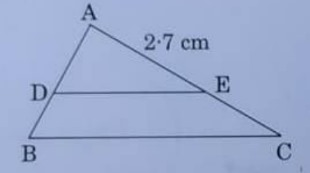
\includegraphics[width=0.5\columnwidth]{figs/Construction-1.jpg}
		\caption{}
	\end{figure}

\item In Figure-2 ,if $PQ || BC$ and $PR || CD$ that $\frac{QB}{AQ} = \frac{DR}{AR}$.
	\begin{figure}[H]
		\centering
		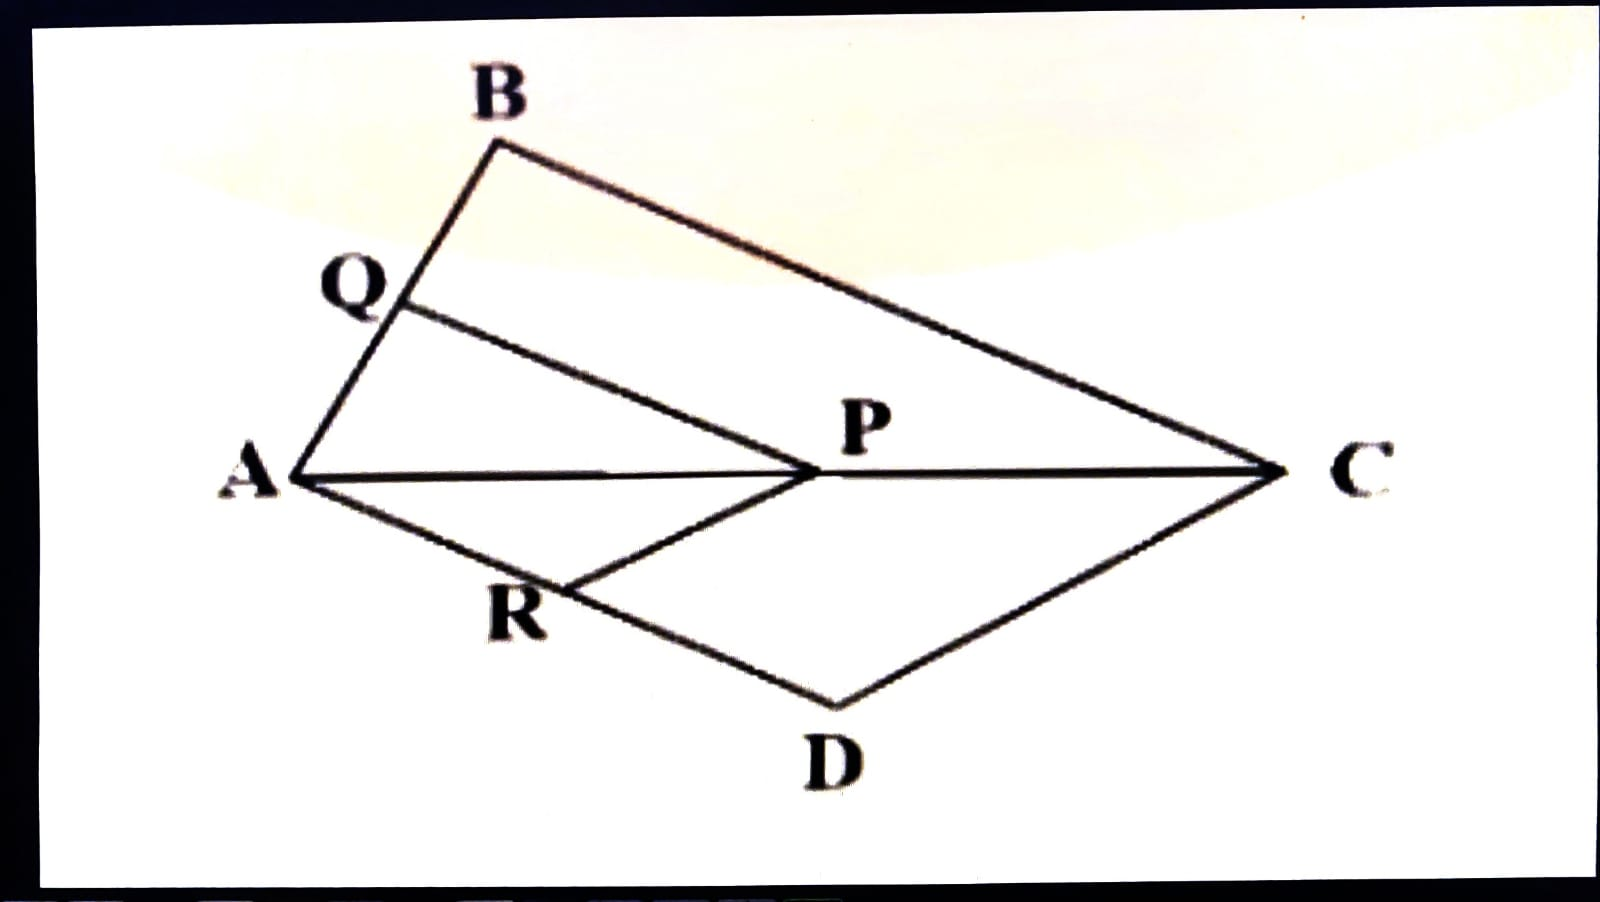
\includegraphics[width=0.5\columnwidth]{figs/Construction-2.jpg}
		\caption{}
	\end{figure}

\end{enumerate}
\end{document}

